Este documento describe la resolución del \textbf{Academy Re-Win -- Entrance Challenge}, el reto de ingreso de Gecko Academy (Binary Gecko). El desafío es un único binario de Windows que presenta \textbf{cuatro niveles encadenados} de ingeniería inversa: cada nivel solo se desbloquea al superar el anterior, y la dificultad crece progresivamente desde un \emph{keygen} clásico hasta una máquina virtual con su propio \emph{bytecode}.

El objetivo de cada nivel no es adivinar una contraseña, sino \textbf{entender el algoritmo de validación} a partir del código desensamblado y reproducirlo, de modo que se pueda generar una credencial válida para cualquier entrada.

\subsection{Estructura del reto}

\begin{table}[H]
\centering
\rowcolors{2}{TableBgRowColor}{TableBgRowIntemediaColor}
\begin{tabularx}{\linewidth}{c l X l}
\rowcolor{TableHeaderBgRowColor}
\textcolor{white}{\textbf{Nivel}} & \textcolor{white}{\textbf{Dificultad}} & \textcolor{white}{\textbf{Qué se pide}} & \textcolor{white}{\textbf{Estado}} \\
1 & Media & Usuario y serial de 8 dígitos hexadecimales derivado del usuario (\emph{keygen}). & Resuelto \\
2 & -- & Serial con formato \texttt{XXXX-XXXX-XXXX-YYYY}, calculado a partir del mismo usuario del nivel 1. & Resuelto \\
3 & Difícil & \emph{Login}: usuario elegido libremente (mínimo 5 caracteres) y su contraseña. & Resuelto \\
4 & Muy difícil & Contraseña validada por una máquina virtual interna; hay que entender su \emph{bytecode}. & Pendiente \\
\end{tabularx}
\caption{Niveles del Academy Re-Win Entrance Challenge}
\end{table}

\subsection{Resultados obtenidos}

La Figura~\ref{fig:levels} muestra la ejecución del reto con las credenciales generadas: los niveles 1 a 3 se superan y el binario desbloquea el nivel final.

\begin{table}[H]
\centering
\rowcolors{2}{TableBgRowColor}{TableBgRowIntemediaColor}
\begin{tabularx}{\linewidth}{c X X}
\rowcolor{TableHeaderBgRowColor}
\textcolor{white}{\textbf{Nivel}} & \textcolor{white}{\textbf{Entrada}} & \textcolor{white}{\textbf{Credencial válida}} \\
1 & Usuario: \texttt{mati} & Serial: \texttt{00389E38} \\
2 & Usuario: \texttt{mati} (heredado) & Serial: \texttt{E834-69B6-1B27-9AA5} \\
3 & Usuario: \texttt{fierro} & Contraseña: \texttt{C65715F2BE5918C4} \\
4 & -- & \emph{En análisis} \\
\end{tabularx}
\caption{Credenciales válidas generadas}
\end{table}

\begin{figure}[H]
\centering
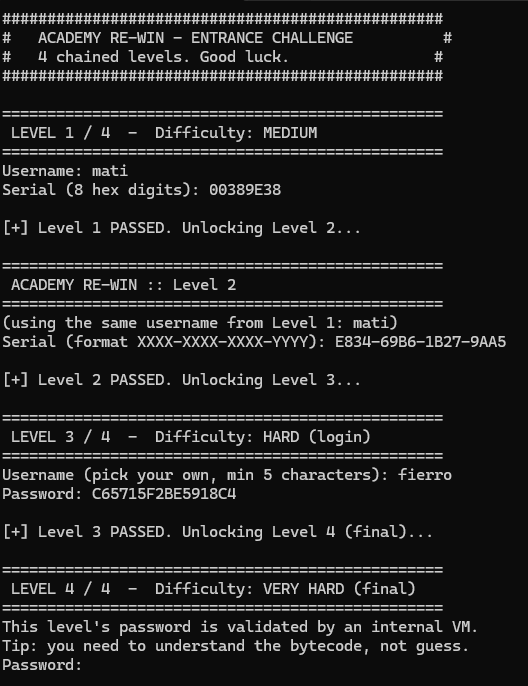
\includegraphics[width=0.55\linewidth]{initial/img/levels.png}
\caption{Ejecución del reto: niveles 1 a 3 superados}
\label{fig:levels}
\end{figure}

\subsection{Metodología y herramientas}

Para cada nivel se siguió el mismo proceso:

\begin{enumerate}
    \item \textbf{Reconocimiento:} ejecutar el binario, observar los mensajes y el formato de entrada esperado.
    \item \textbf{Análisis estático:} ubicar la rutina de validación en el desensamblador a partir de las cadenas de texto y las llamadas de entrada/salida.
    \item \textbf{Análisis dinámico:} confirmar el comportamiento con un depurador, colocando \emph{breakpoints} en la comparación final.
    \item \textbf{Reconstrucción del algoritmo:} reescribir la validación en un lenguaje de alto nivel.
    \item \textbf{Keygen y verificación:} generar credenciales para usuarios arbitrarios y comprobarlas contra el binario.
\end{enumerate}

% TODO: ajustar la lista de herramientas a las realmente usadas
Herramientas utilizadas: \emph{Ghidra / IDA} (análisis estático), \emph{x64dbg} (análisis dinámico) y \emph{Python} (keygens).
